\documentclass[]{standalone}

\usepackage{graphicx}
\usepackage[linesnumbered,ruled,vlined]{algorithm2e}
\usepackage{color,soul}
\usepackage[utf8]{inputenc}
\usepackage[T1]{fontenc}
\usepackage{textcomp}
\usepackage{amsmath, amssymb}
\usepackage{caption}
\usepackage{listings}

% figure support
\usepackage{tikz}
\usetikzlibrary{calc}
\usepackage{import}
\usepackage{xifthen}
\pdfminorversion=7
\usepackage{pdfpages}
\usepackage{transparent}
\usepackage[hidelinks]{hyperref}

\pdfsuppresswarningpagegroup=1

\begin{document}
	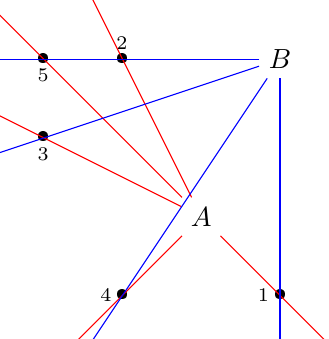
\begin{tikzpicture}[>=stealth]
		\node[] (A) at (3,2) {$A$};
		\node[] (B) at (4,4.0) {$B$};
		\node[] (1) at (4,1) {\textbullet};
		\node[] (2) at (2,4) {\textbullet};
		\node[] (3) at (1,3) {\textbullet};
		\node[] (4) at (2,1) {\textbullet};
		\node[] (5) at (1,4) {\textbullet};
		\node[left] (11) at (1) {$_1$};
		\node[above] (12) at (2) {$_2$};
		\node[below] (13) at (3) {$_3$};
		\node[left] (14) at (4) {$_4$};
		\node[below] (15) at (5) {$_5$};

		\draw[color=red, shorten >=-200] (A) -- (1);
		\draw[color=red, shorten >=-200] (A) -- (2);
		\draw[color=red, shorten >=-200] (A) -- (3);
		\draw[color=red, shorten >=-200] (A) -- (4);
		\draw[color=red, shorten >=-200] (A) -- (5);

		\draw[color=blue, shorten >=-200] (B) -- (1);
		\draw[color=blue, shorten >=-200] (B) -- (2);
		\draw[color=blue, shorten >=-200] (B) -- (3);
		\draw[color=blue, shorten >=-200] (B) -- (4);
		\draw[color=blue, shorten >=-200] (B) -- (5);
		
		
		
	\end{tikzpicture}
\end{document}
